\section{Introduction}

Searches for various BSM theories including SUSY have been performed at LHC  alongside searching for the Higgs and performing different SM anlyses. Many SUSY searches were conducted targeting the production of squarks and gluinos. This was motivated by a larger theoretical cross-section and therefore higher probability of producing coloured superpartners \cite{borschensky2014squark}. Up to this moment no statistically significant excess over SM has been detected and exclusion limits were placed on masses of SUSY particles. Figure~\ref{fig:SUSYlimit} shows the latest data on the masses that have been excluded for supersymmetric particles in various production scenarios. The lower limits on the masses of most squarks and gluinos in different searches significantly exceed 1 TeV \citep{aad2015summary}. As a consequence, if their production occurs, it is either extremely rare at present energies or requires higher energy of collision to leave an identifiable signature. 

This thesis's research will focus on the electroweak production as one of the possible SUSY particle production scenario. Sleptons and gauginos are produced in electroweak production processes and are not affected by the strong force. They have smaller cross-sections compared to squarks and gluinos, so their theoretical production rate is smaller. However, if their masses are small compared to the strongly interacting sparticles, SUSY production will likely be dominated by electroweak production where sparticles have smaller mass and current energy might be enough to produce them in quantities that would allow their detection \citep{aad2016search}.
%\newgeometry{left=1cm,right=1cm}
\begin{figure}[!ht]
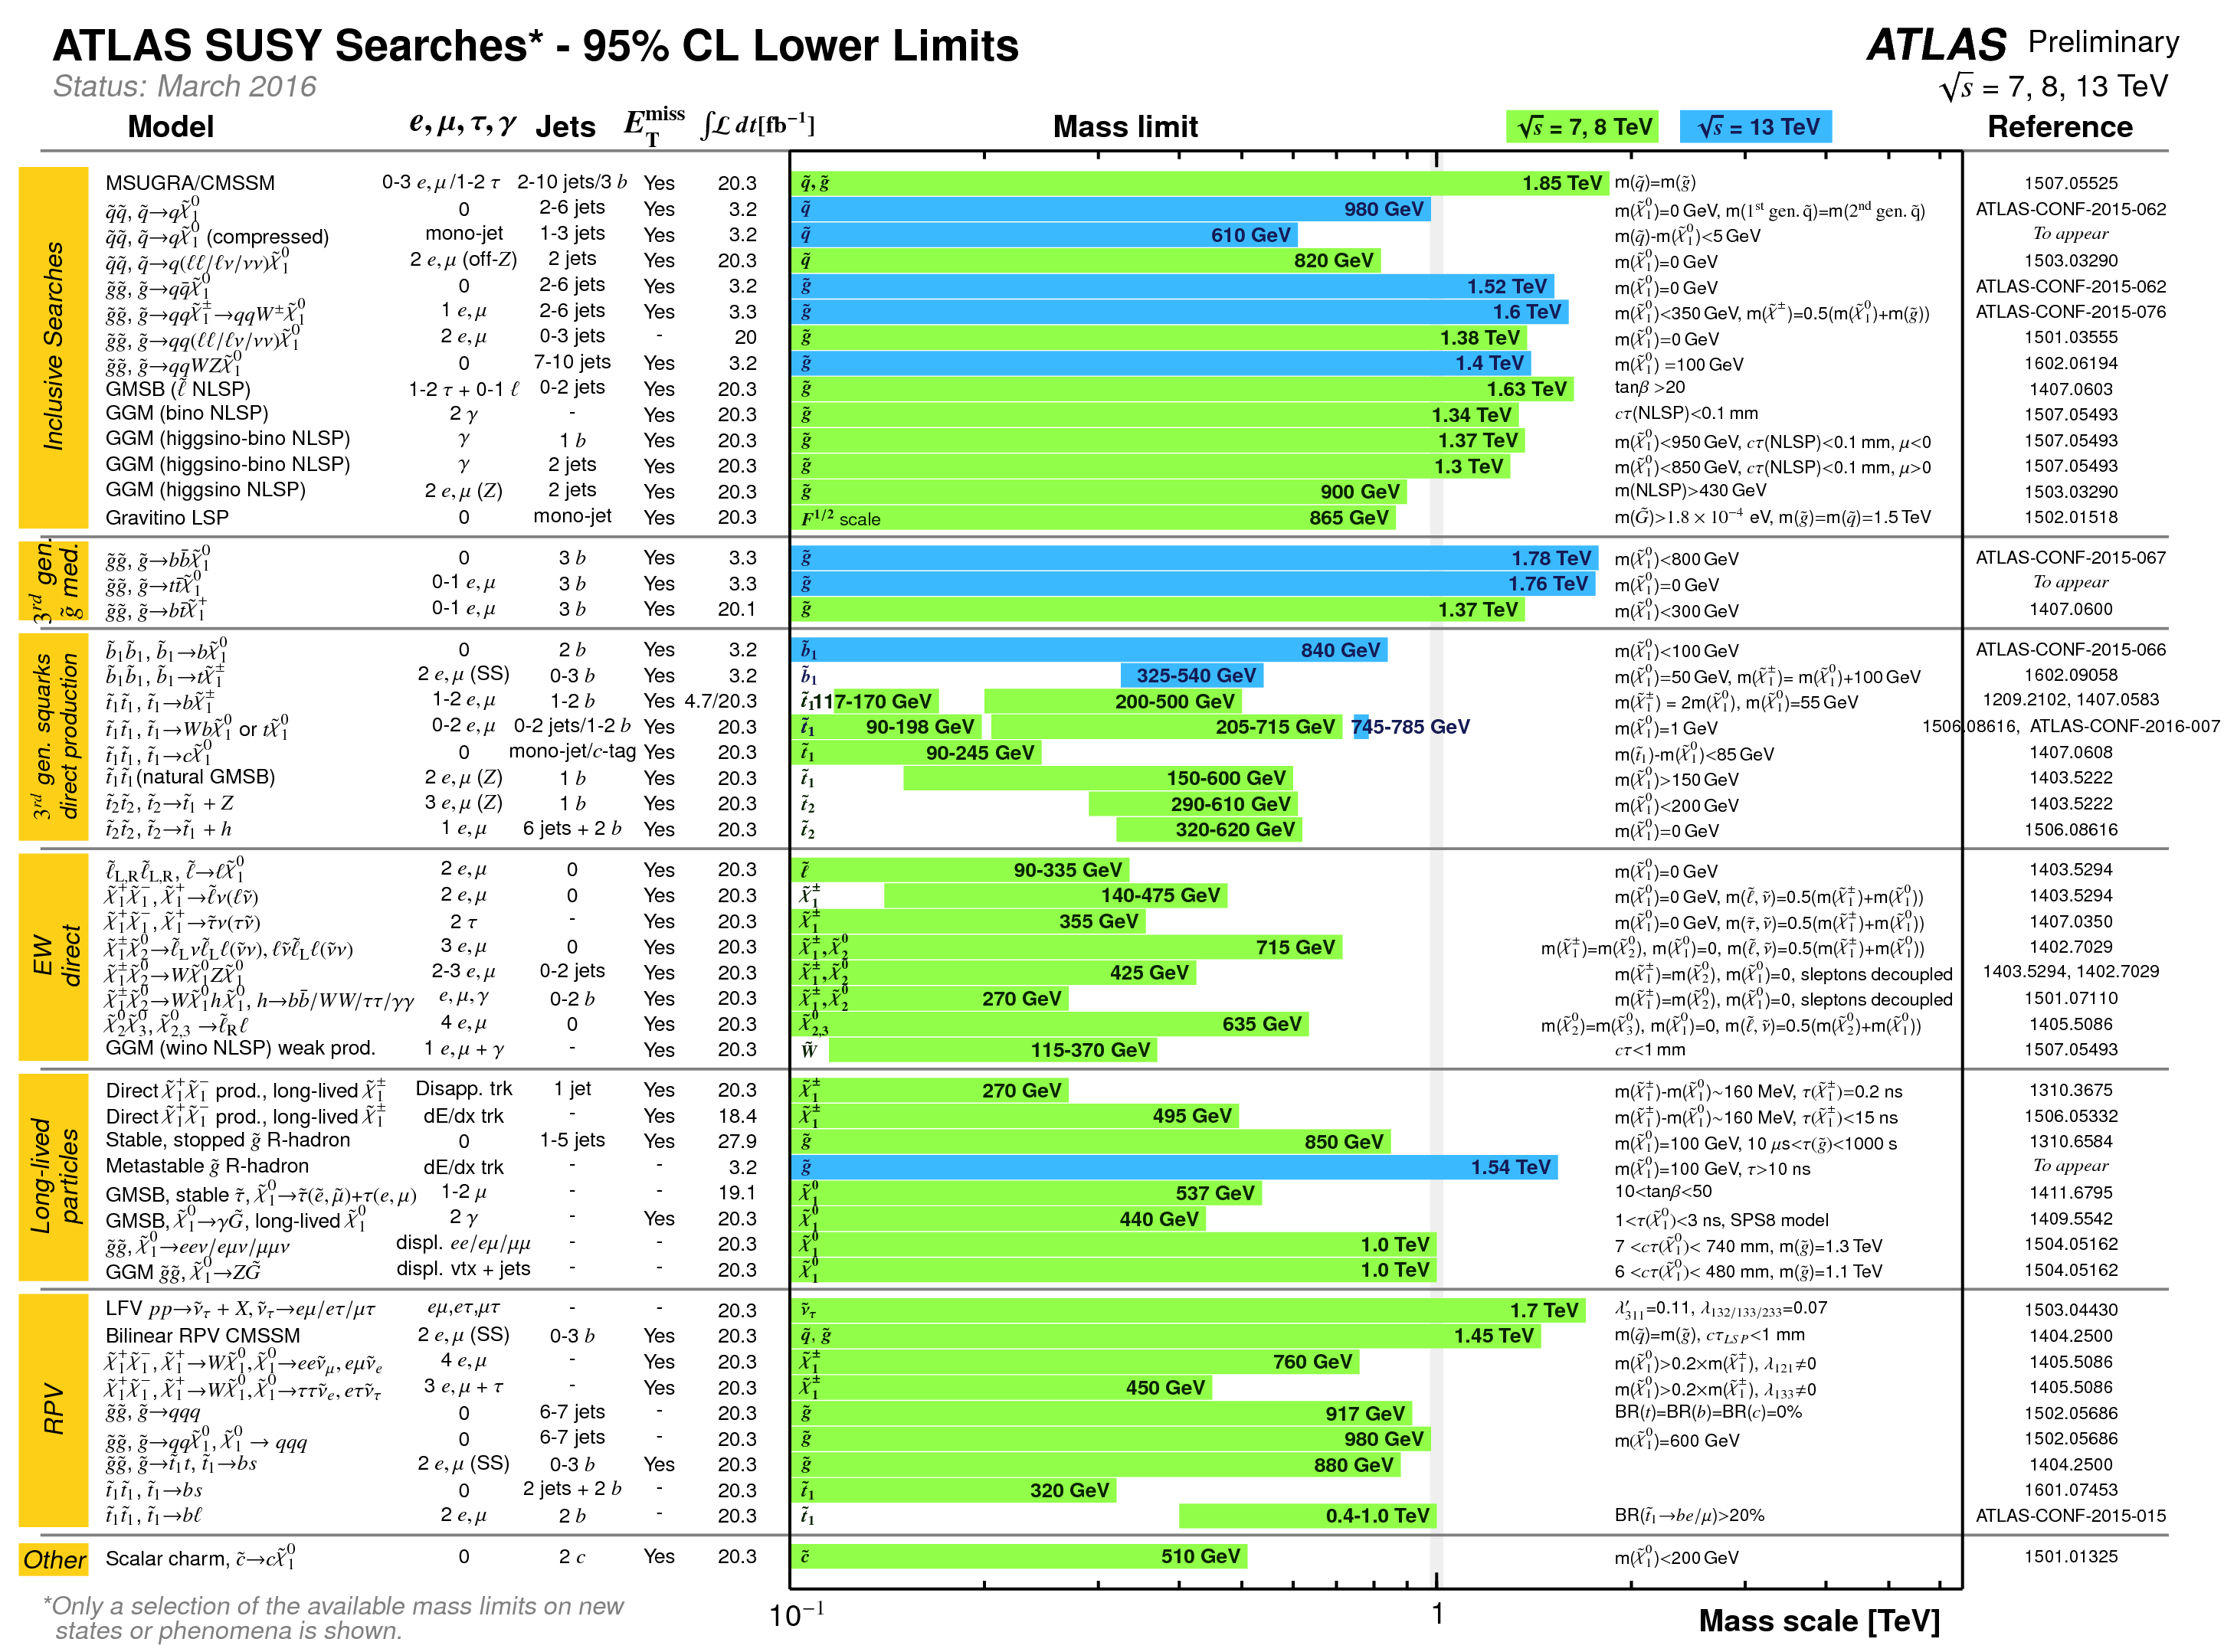
\includegraphics[width=\textwidth]{Chap3/ATLAS_SUSY_Summary.png}
\caption{Exclusion limits of ATLAS searches for Supersymmetry \citep{SUSYlimits}}
\label{fig:SUSYlimit}
\end{figure}
\cleardoublepage


So far searches in the electroweak region have been unable to find evidence of supersymmetric particles. Limits on their masses according to various decay scenarios have been obtained and can be seen in Fig \ref{fig:summaryplot}.
\begin{figure}[!ht]
	\centering
	\captionsetup{width=0.8\textwidth}
	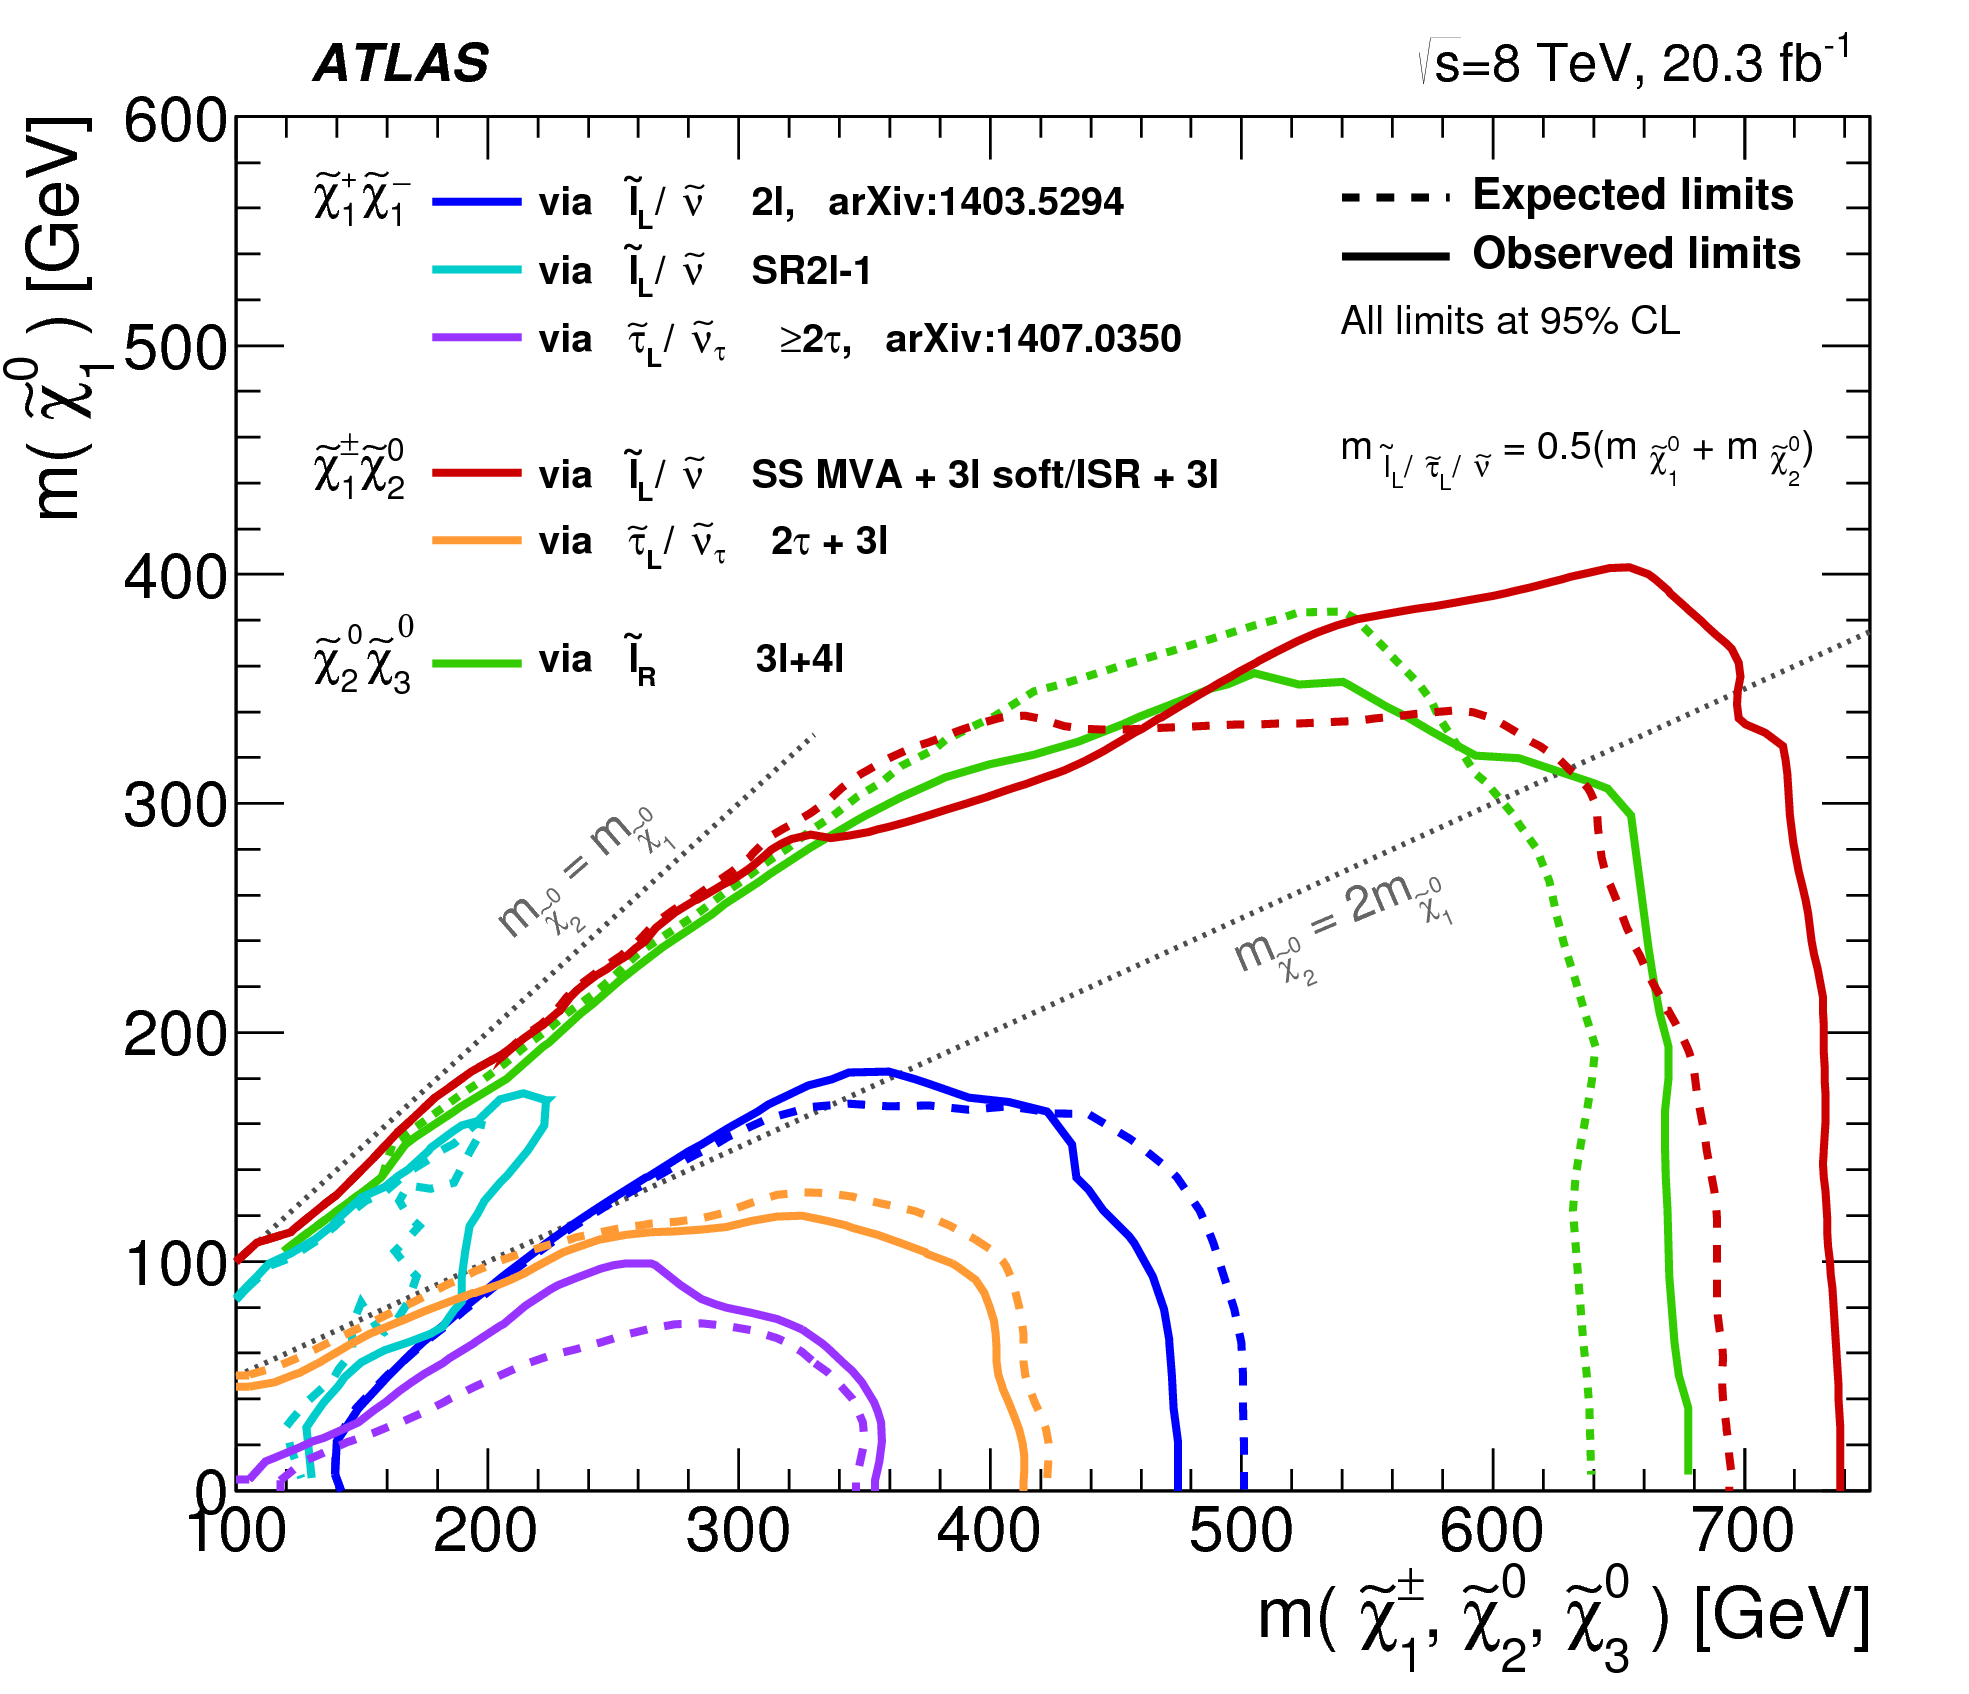
\includegraphics[scale=0.15]{Chap3/fig_19b}
	\caption{The 95\% CL exclusion limits on $\chi_1^+\chi_1^-$, $\chi_1^{\pm}\chi_2^0$ and $\chi_2^0\chi_3^0$ production with $l$-mediated decays, as a function of the $\chi_1^{\pm},\,\chi_2^0$ and $\chi_1^0$ masses \citep{aad2016search}. }\label{fig:summaryplot}
\end{figure}

These results are taken from \citep{atlas2015search} analysis performed at $\sqrt{s}=$8 TeV and integrated luminosity of 20.3 fb\textsuperscript{-1}. This search was performed based on various scenarios of the pMSSM, involving electroweak production of charginos and neutralinos. The turquoise and blue lines represent decay scenarios that are relevant for this paper as they show information on slepton-mediated decays of a chargino pair. 
In particular, the production of $\tilde{\chi}^{+}_{1}\tilde{\chi}^{-}_{1}$ pair decaying through a slepton ($\tilde{l}$) with final states contatining two opposite sign leptons will be considered (see Fig. \ref{fig:EWchargino}). 
\begin{figure}[!h]
  \centering   	
  	\captionsetup{width=0.8\textwidth}
	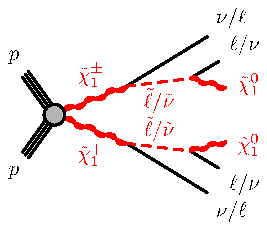
\includegraphics[]{Chap2/C1C1-llvvN1N1-slsnu}	
\caption[Optional caption for list of figures]{Electroweak chargino pair production in proton-proton collisions with intermediate slepton in the decay process.}\label{fig:EWchargino}
\end{figure}  

In the nomenclature used at LHC and in this thesis, electrons and muons are called "light leptons". Taus are considered separately as they decay very promptly and therefore are very difficult to reconstruct. This thesis only focuses on final states containing electrons and muons and the designation "lepton" only refers to these particles.  


%However, given that so far only 3.2 fb\textsuperscript{-1} of integrated luminosity has been achieved at $\sqrt{s} = 13$ TeV.

\subsection{Search methods}
Detecting new physics events at LHC requires using computational and statistical methods that can deal with the type of information a particle accelerator produces. The data is initially collected using triggers corresponding to the type of events under analysis. Each event has a large number of physical characteristics such as momentum, energy, mass, multiplicities, etc. The numbers representing them are all stored in a data structure which then can be accessed, modified and analysed using software tools. 

The cornerstone of all accelerator physics analyses is the correct estimation of background events. All background events represent physics that is already known and that has some similar or identical features with the processes we wish to study. For instance, this thesis focusses on the  reactions that have precisely two oppositely charged leptons in their final states. A number of processes well described by the standard model share this characteristic and therefore will form the background. 

The presence or absence of a new particle also can reveal itself in a number of ways. The case that is the easiest to detect is when there is an abnormality in mass distribution, such as the case with Higgs particle discovery. The peak in mass distribution of diphoton events constituted a significant excess over SM predictions \citep{chatrchyan2012observation,Aad:2012tfa}. 

This method does not work for SUSY particles and other techniques have to be used. Standard search techniques involve defining \textbf{signal regions} in data distributions that are sensitive to possible SUSY signals and looking whether there is a significant excess over SM background predictions in these regions. Another method is looking for abnormal tails in distributions that are not in agreement with SM predictions.   


%The overall goal is to have a procedure that loops over all events and selects those that are of interest for further analysis. 